\documentclass[10pt,a4paper]{article}
\usepackage[utf8]{inputenc}
\usepackage[english]{babel}
\usepackage[T1]{fontenc}
\usepackage{amsmath}
\usepackage{amsfonts}
\usepackage{amssymb}
\usepackage{subcaption}
\usepackage{makeidx}
\usepackage{graphicx}
\usepackage{fourier}
\usepackage{listings}
\usepackage{color}
\usepackage{hyperref}
\usepackage[left=2cm,right=2cm,top=2cm,bottom=2cm]{geometry}
\author{Tommy Müller, Marcus Dittrich, Vincent Noculak}
\title{ Mie-Streuung an levitierten Flüssigkeitströpfchen}


\begin{document}

\maketitle
\newpage
\tableofcontents
\newpage

\section{Einleitung}

In dem Versuch, Mie-Streuung an levitierten Flüssigkeitströpfchen, soll die Streuung von Laserlicht an kleinen Glaskügelchen und Aerosoltröpfchen untersucht werden. Der Radius der Kügelchen ist in der Größenordnung der Lichtwellenlänge. Diese geladenen Teilchen werden in einer Paulfalle in schwebe gehalten. Das verdampfen der Aerosoltröpfchen kann ebenso beobachtet werden.

\section{Theorie}
\subsection{Paulfalle}

Wir betrachten ein Teilchen mit der Masse m und der Ladung q im Potenzial\\

$\Phi(\overrightarrow r) = V (\alpha x^2+\beta y^2+\gamma z^2)$\\
Am Anfang betrachten wir den Raum als ladungsfrei, daher gilt die Laplace - Gleichung.\\
\begin{equation}
\Delta \Phi = 0   \leftrightarrow \alpha + \beta + \gamma = 0
\label {1}
\end{equation}
Es gibt viele Lösungen für die Gleichung, eine mögliche Lösung ist:

$$\alpha = \beta\ und\ \gamma = -2 \alpha$$
Mit dieser Wahl erhalten wir das Potenzial

\begin{equation}
\Delta \Phi = \frac{V}{2r_0^2}(r^2-2z^2)
\label {2}
\end{equation}
Dieses Potenzial ist nach \ref {1} für konstantes Potenzial, es gibt keinen Ort mit minimalen Potenzials. Ändert man nun V in V = V (t)= U-$V_0 \cos(\omega t)$ so ist damit die Konstruierung einer Teilchenfalle möglich. \\ \\Die Bewegungsgleichung des Teilchens in z- und r- Richtung sind mit $\overrightarrow F = - Q \delta\overrightarrow \phi$ gegeben durch

\begin{equation}
\frac {d^2r}{dt^2} = \frac{Q}{r_0^2 m}(U-V_0 \cos(\omega t)r)
\label {3}
\end{equation}


\begin{equation}
\frac -{1}{2}\frac {d^2z}{dt^2} = \frac{Q}{r_0^2 m}(U-V_0 \cos(\omega t)z)
\label {4}
\end{equation}
Nach dem einsetzen erhalten wir zwei Differenzialgleiungen 


\begin{equation}
a_z = -2a_r =\frac{-8 Q U}{r_0^2 m \omega^2}\
,q_z = -2q_r =\frac{-4 Q V_0}{r_0^2 m \omega^2}; 2\epsilon = \omega t
\label {5}
\end{equation}
die Form der Mathieuschen Differenzialgleichung \\

$$ f``(\epsilon) + (a-2b \cos(2\epsilon))f(\epsilon) = 0$$\\
Die Lösungen der Mathieuschen  Differenzialgleung sind bekannt. Diese ist in allgemeiner Form gegeben durch: \\\\

$$ f(\epsilon) = A e^{\mü \epsilon} \sum_{\infty}^\infty C_{2n} e^{i2n\epsilon}+B e^{-\mü \epsilon} \sum_{\infty}^\infty C_{2n} e^{-i2n\epsilon}$$\\Nun ist die Frage, ob die Teilchenbahn stabil ist, d.h. ot r(t) und z(t) in einem gewissen Abstand nicht überstreiten, für dies muss Re($\mü$) = 0 gelten. 
Die Größen für die Stabilitätsbedingung sind die Masse m, Ladung q sowie die Spannungen U und $V_0$, diese ergeben das Stabilitätsdiagramm. In Abbildung \ref{stab} wurde a über q aufgetragen, der stabile Bereich ist durch die Funktionsgraphen eingegrenzt. Der Bereich gilt nur für den idealisierten Fall im Vakuum. Die stabilen Bereiche würden sich ausweiten wenn man die viskose Dämpfung (z.B. Luftreibung)  mit einbezieht. Sind die Stabilitätsbedingungen passend, so lässt sich ein Teilchen in der Falle unbegrenzt lange im Koodinatenursprung halten.


\begin{figure}[h]
	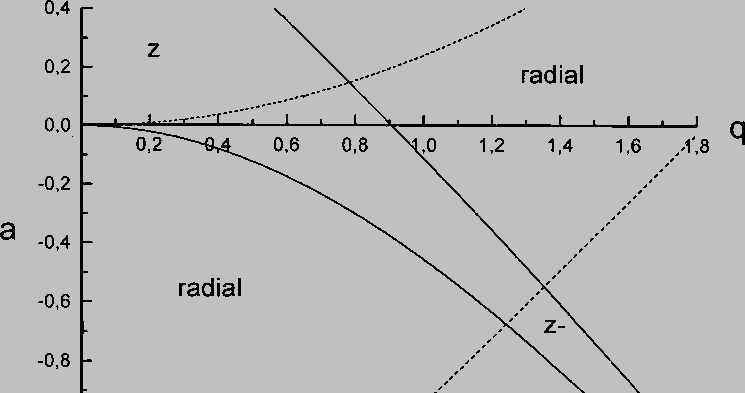
\includegraphics[scale = 0.5]{Paulstabdia.png}
	\centering
	\caption{Stabilitätsdiagramm einer Paulfalle}
	\label{stab}
\end{figure}



\subsection{Mie-Streuung}

Mie-Streuung bezeichnet Streuung von Licht an  sphärischen, homogenen Partikeln. Im Grenzfall großer Radien bekommt man die Gesetze der geometrischen Optik, für kleine Radien die Rayleight-Streuung. Die Mie-Streuung ist beschränkt auf Teilchen mit dem Durchmesser von der Größenordnung der Wellenlänge des verwendeten Lichtes.
Größenparameter ist hierbei k= $\frac {2\pi r}{\lambda}$, ist dieser in der Größenordnung von 1 bilden sich ein Beugungsmuster aus, deren Maxima und Minima vom Größenparameter abhängt.
Die theoretischen Probleme der Lichtstreuung an solch einem Partikel besteht im wesentlichen aus der Lösung der Maxwell-Gleichung mit Stetigkeitsbedingungen an dessen Oberfläche. Ein Ergebniss ist das die Intensitätsverteilung sowie Minima und Maxima rückschlüsse auf den Brechungsindex des Partikels und dessen Abmessungen geben.

\subsection{Verdampfungsprozess}

Die Verdampfung von Teilchen bei T = konst. beschreibt die Teilchendiffusion. Folgende Differenzialgleichung lässt sich für den Radius des Teilchen aufstellen:\\

$\frac{dr}{dt}= -\frac {S}{2r} \leftrightarrow \frac {d}{dt}r^2(t)=-S$
Der Verdampfungsparameter S ist hierbei von der Umgebungstemeratur und dem Druck abhängig. Nun Integriert man die Differetialgleichung und so erhält man eine Gleichung für die Oberfläche des Teilchen in Abhängigkeit von $r_0$ Radius zum Zeitpunkt $t_0$. 

\begin{equation}
r^2(t)= r_0^2-S(t-t_0)
\label {6}
\end{equation}





\subsection{Bestimmung der Massenlandungsdichte Q/m}

Ein geladenes Teilchen das sich in Ruhe in einem elektrischen Feld befindet, hierbei kompensiert die Gewichtskraft genau die Coulomb-Kraft.\\


$F_{Gewicht}=F_{Coulomb}$
\\
Die Gewichtskraft ist $F_{Gewicht}=mg$. Die Coulomb-Kraft eines homogenen elektrischen Feldes muss mit Hilfe eines Korrekturfaktors genähert werden (K=0.798). \\

$F_{Coulomb}=Q\frac{U}{2z_0}K=Q\frac{U}{\sqrt2 r_0}0.798$

Jetzt setzt man nun beide Kräfte gleich und dann folgt für Q/m mit $r_0 $ und g = 9.81 $\frac{m}{s^2}$:

\begin{equation}
\frac{Q}{m}=\frac{\sqrt2 r_0 g}{0.798 U}
\label {7}
\end{equation}

\section{Versuchsaufbau}

Der Versuchsaufbau besteht aus einer Paulfalle, einem Helium-Neon-Laser und einer digitalen Videokamera. Der Laserstrahl wird auf das Zentrum der Paulfalle gerichtet und das Streulicht mit der Kamera aufgenommen. Die Streulichtintensität wird dann mit einem Computerprogramm analysiert.

\begin{figure}[h]
	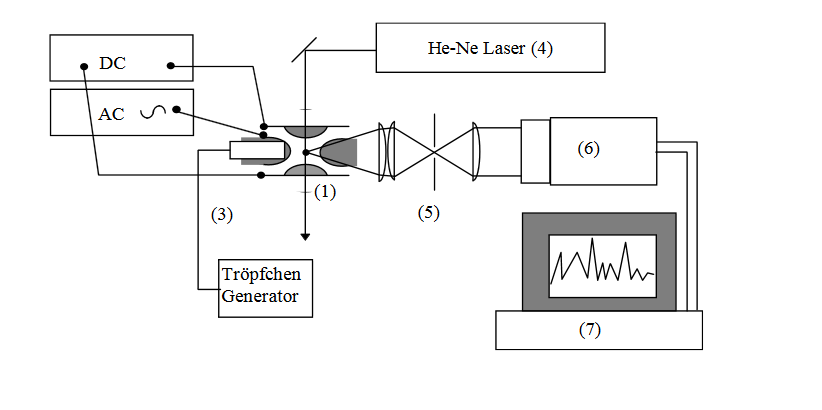
\includegraphics[scale = 0.5]{aufbau.png}
	\centering
	\caption{ Skizze des Versuchsaufbaus, mit den Komponenten (1) Paulfalle, (3) PiezoInjektor, (5) Linsensystem, (6) CCD-Kamera und (7) Messcomputer}
	\label{aufbau}
\end{figure}

\section{Durchführung}

\subsection{Versuchsdurchführung}
Zunächst wurde die Falle mit einer angelegten Wechselspannungsamplitude von 250 V mit
einer Frequenz von 100 Hz in Betrieb genommen. Dann wurden die Glaskügelchen mittels
eines Glasstäbchens in die Paulfalle gebracht. Das Bild der Kamera zeigte den mit
einem HeNe-Laser beleuchteten Probenbereich der Falle und die Kügelchen, die durch die
Falle fielen. Um die Kügelchen zu fangen, wurde die Gleichspannung zwischen Deckel und
Bodenelektrode variiert.
Nach ein paar Versuchen konnten mehrere Glaskugeln in der Falle gefangen werden.
Bei Erhöhung der Gleichspannung U wurde das Teilchen nach oben verschoben. Diese Glaskügelchen haben wir mit dem Programm view mie scattering.vi auf dem PC angesehen und Spannungen aufgenommen als diese in schwebe waren. Wir konnten von 3 Glaskügelchen den Q/m Wert bestimmen. Als nächstes entfernten wir die Glaskügelchen aus der Falle und erzeugten mit einer piezoelektrisch betriebene Düse Aerosoltröpchen um die Verdampfungskonstante zu bestimmen. Davor brauchten wir jedoch den Mittelpunkt der Aufnahme sowie Breite. Die Beleuchtung der levitierten Teilchen erfolgt durch einen HeNe-Laser. Die Verdampfungskonstante haben wir an 2 Teilchen bestimmt und diese eine Zeit lang beobachtet bis das Teilchen weg war.


\subsection{Eichkurve}

Die für den Versuch angezeigte Wechselspannung der Ringelektrode entsprach nicht der tatsächlich angelegten Spannung. Deshalb musste vor der Messung eine Eichkurve gemessen werden. Die gemessene Eichkurve ist in Abbildung \ref{eichkurve1} zu sehen. Es kann ein linearer Zusammenhang zwischen der abgelesenen und tatsächlich angelegten Spannung erkannt werden. Mit der Methode der kleinsten Quadrate wurde eine Ausgleichsgerade durch die Messwerte gelegt. Mit dieser Methode wurde auch der Fehler der Steigung der Geraden abgeschätzt. Die Steigung der Ausgleichsgerade beträgt $0,0824 \pm 0,0002$. Wegen dem linearen Zusammenhang muss beim Ablesen einer Spannung diese nur mit der Steigung der Ausgleichsgerade multipliziert werden, um die angelegte Spannung zu berechnen.

\begin{figure}[h]
	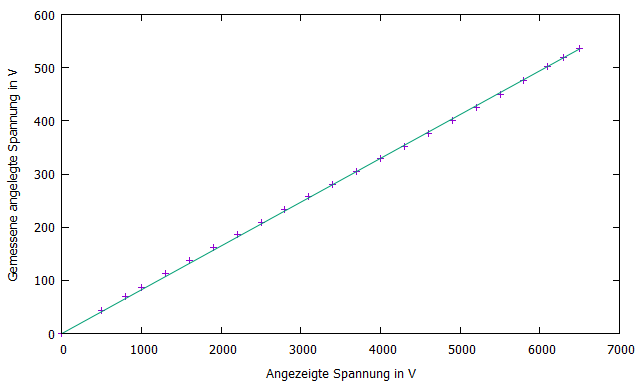
\includegraphics[scale = 0.7]{eichkurve.png}
	\centering
	\caption{Eichkurve der angelegten Wechselspannung an der Ringelektrode; Steigung der Ausgleichsgerade: $0,0824 \pm 0,0002$}
	\label{eichkurve1}
\end{figure}

\section{Versuchsauswertung}

\subsection{Q/m-Werte gefangener Glaskugeln}

Wir haben versucht, geladene Glaskügelchen stabil in der Paul-Falle gefangenzuhalten. Dies ist nur bei zwei Kügelchen für mehr als eine Spannungseinstellung gelungen. Die gemessenen Kugeln können in Tabelle \ref{gefangen} gesehen werden. Zum berechnen des $\frac{Q}{m}$-Verhältnisses der beiden Kugel müssen wir die Spannungen der Deckel- und Bodenelektrode betrachten.\\\\Eine numerische Berechnung des $\vec{E}$-Feldes in der Mitte der Paul-Falle ist aus der Versuchsanleitung vorgegeben als 

\begin{equation}
	E_{Mitte} = \frac{0,798 \cdot (U_{Deckel} - U_{Boden})}{2 z_0}
	\label{emitte1}
\end{equation}
$z_0$ ist der Abstand von der Mitte bis zum Boden/zur Decke der Paul-Falle. Wenn das E-Feld die Gravitationskraft eines Glaskügelchens kompensiert, muss gelten

\begin{equation}
	Q E = m g
\end{equation}
Daraus folgt durch Einsetzen von \eqref{emitte1}

\begin{equation}
	\frac{Q}{m} = \frac{2 z_0 g}{0,798 \cdot(U_{Deckel} - U_{Boden})}
	\label{mqformel1}
\end{equation}
Der Abstand zwischen Boden- und Deckelelektrode ist als $\frac{10}{\sqrt{2}}mm$ gegeben. Somit folgt $z_0 = \frac{5}{\sqrt{2}}mm$.\\Der mithilfe von \eqref{mqformel1}, mit den Werten aus Tabelle \ref{gefangen}, berechnete Wert von $\frac{Q}{m}$ ist für Kugel Nummer 1 $(4,6 \pm 0,4)*10^{-3} \frac{kg}{C}$. Die Standardabweichung wurde als Fehler genommen. Für Kugel Nummer 2 lässt sich $\frac{Q}{m}$ nicht berechnen, weil Deckel- und Bodenspannung identisch sind. Weil für kleinere Differenzen von $U_{Deckel}$ und $U_{Boden}$ $\frac{Q}{m}$ größer wird, kann man vermuten, dass Kugel Nummer 2 einen großen Wert für $\frac{Q}{m}$ hat. Weil wir nur für eine Kugel den Wert für $\frac{Q}{m}$ bestimmen konnten, ist es uns nicht möglich, Aussagen darüber zu treffen, in welchen Bereichen die Werte für die spezifische Ladung der Glaskügelchen liegen.

\begin{table}[h!]
	\centering
	\begin{tabular}{|l|l|l|l|l|}\hline
		Kugelnummer & $U_{Deckel}$/V ($\pm 1V$)& $U_{Boden}$/V ($\pm 1V$)& $U_{Ring}$/V ($\pm 1V$)& Wechselspannungsfrequenz f/Hz\\\hline
		1 & 158 & 142 & 267 & 101\\
		1 & 161 & 140 & 306 & 101\\
		1 & 160 & 141 & 317 & 101\\
		1 & 161 & 140 & 286 & 101\\
		2 & 150 & 150 & 323 & 101\\
		2 & 150 & 150 & 292 & 101\\\hline
	\end{tabular}
	\caption{Messwerte für in der Paul-Falle gefangene Glaskügelchen}
	\label{gefangen}
\end{table}

\subsection{Stabiler Bereich im a/q-Raum}
Wir betrachten die Werte für a und q, bei denen die Glaskügelchen unserer Messungen stabil waren. Als Stabilitätskriterium der Kügelchen hatten wir festgelegt, dass die Amplitude, in der sie oszillieren, kleiner gleich ihrem zweifachen Durchmesser sein muss. a und q lassen sich mit folgenden Formeln berechnen:

\begin{equation}
	a = -8 \frac{Q}{m} \frac{U}{r_o^2 (2 \pi f)^2}
\end{equation}
\begin{equation}
	q = -4 \frac{Q}{m} \frac{V_0}{r_0^2 (2\pi f)^2}
\end{equation}
Der Durchmesser der Ringelektrode ist mit $10mm$ gegeben. Daraus ergibt sich $r_0 = 5mm$.\\\\Für die zweite Kugel war die spezifische Ladung nicht zu berechnen, weshalb wir nur den stabilen Bereich der ersten Kugel betrachten können. In Tabelle \ref{gefangen2} sind die benötigten gemessenen Werte zur Berechnung von a und q angegeben. Die daraus berechneten Werte sind ebenfalls in der Tabelle zu sehen. \\\\Wir tragen die erhaltenen Werte für a und q in ein Diagramm ein und untersuchen, ob die Werte in dem theoretisch vorhergesagten stabilen Bereich liegen. Die Grenzen des ersten Stabilitätsbereiches des Stabilitätsdiagramms sind durch folgende Kurven gegeben:
\begin{align}
	a(q) = - \frac{1}{2} q^2 + \frac{7}{128} q^4 - \frac{29}{2304} q^6 + \frac{68687}{18874368}\\
	a(q) = 1-q-\frac{1}{8} q^2 + \frac{1}{64} q^3 - \frac{1}{1536} q^4 - \frac{11}{35864} q^5	
\end{align}
Weil die Stabilität nur von Betrag für q anhängt, spiegeln wir unsere q-Werte am Nullpunkt, bevor wir das Diagramm erstellen. \\\\Das erhaltene Diagramm für unsere Messwerte im Stabilitätsdiagramm kann in Abbildung \ref{stabiler_bereich1} gesehen werden. Alle a/q-Wertepaare liegen innerhalb des theoretisch vorhergesagten stabilen Bereiches. Auch die dreifachen Fehlerintervalle der Messwerte liegen noch im stabilen Bereich. Es fällt auf, dass alle Messwerte sehr zentral und nah aneinander liegen. Experimentell hatten wir beobachtet, dass die Kügelchen sehr schnell labil wurden und aus der Paul-Falle entkamen. Dies ist beim Betrachten der Werte im Diagramm, die zu unserer ersten beobachteten Kugel gehören, widersprüchlich. Laut dem Diagramm hätten wir die angelegte Gleich- oder Wechselspannung noch etwas verändern können, ohne dass die Kugel instabil wird. Das war uns nicht möglich. Folglich erreichten wir mit unseren Messwerten auch nicht die theoretische Grenze des stabilen Bereiches.\\\\Da alle unsere Messwerte im theoretisch vorhergesagten Bereich des Stabilitätsdiagramms liegen, kann angenommen werden, dass dieser im Grunde für unseren Messaufbau gelten muss. Weil es uns nicht möglich war, mit den Messwerten bis zur Grenze des theoretischen stabilen Bereichs zu gelangen ohne, dass die Kügelchen instabil wurden, ist es möglich, dass der tatsächliche stabile Bereich unseres Versuchaufbaus kleiner, als der theoretisch vorhergesagte ist. \\\\Es muss berücksichtigt werden, dass in die Messdaten nicht zu viel hineininterpretiert werden darf, weil es sich bei ihnen um nur vier Messpunkte handelt. Von vier Messpunkten ausgehend, kann man nur sehr eingeschränkt Aussagen über die Struktur des stabilen Bereiches treffen. 

\begin{table}[h!]
	\centering
	\begin{tabular}{|l|l|l|l|l|l|}\hline
		Kugelnummer & Gleichspannung U/V ($\pm 2V$) & Wechselspannung $V_0$/V ($\pm 1V$)& f/Hz & a & q\\\hline
		1 & 16 & 267 & 101 & $-0,059 \pm 0,009$ & $-0,49 \pm 0,04$\\
		1 & 21 & 306 & 101 & $-0,077 \pm 0,01$ & $-0,56 \pm 0,05$\\
		1 & 19 & 317 & 101 & $-0.069 \pm 0,009$ & $-0.58 \pm 0,05$\\
		1 & 21 & 286 & 101 & $-0,077 \pm 0,01$ & $-0,52 \pm 0,05$\\
		2 & 0 & 323 & 101 &&\\
		2 & 0 & 292 & 101 &&\\\hline
	\end{tabular}
	\caption{Gemessene Spannungen und berechnete Werte für a und q}
	\label{gefangen2}
\end{table}

\begin{figure}[h]
	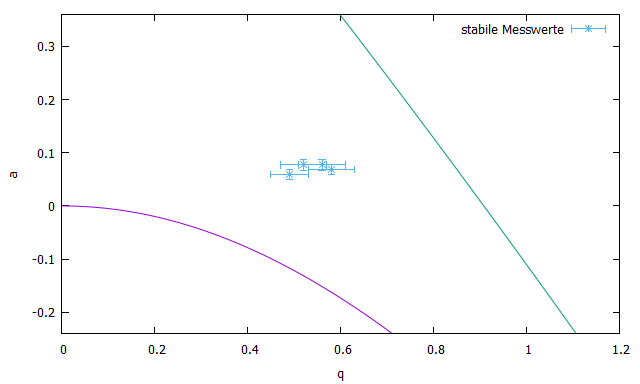
\includegraphics[scale = 0.7]{stabiler_bereich.png}
	\centering
	\caption{Messwerte für stabile Glaskügelchen im Stabilitätsdiagramm}
	\label{stabiler_bereich1}
\end{figure}

\subsection{Verdampfung des Ethanol-Tröpfchen}
Im zweiten Teil unseres Experimentes sollten wir das Verdampfen eines Ethanol-Tröpfchens im Strahl eines He-Ne-Lasers ($\lambda = 632,8 nm$) untersuchen. Zunächst haben wir mittels eines Piezo-Injektors ein Tröpfchen erzeugt und in der Paulfalle gefangen. Um das entstehende Bild in der CCD-Kamera bestmöglich auswerten zu können, haben wir mit der Linse im Strahlengang soweit verschoben, bis das Tröpfchen auf dem Bildschirm im Aufnahmeprogramm größtmöglich zu sehen war. Des weiteren mussten wir den maximal sichtbaren Winkelbereich berechnen, welcher sich aus folgender geometrischen Überlegung ergibt. 
\begin{figure}[h]
	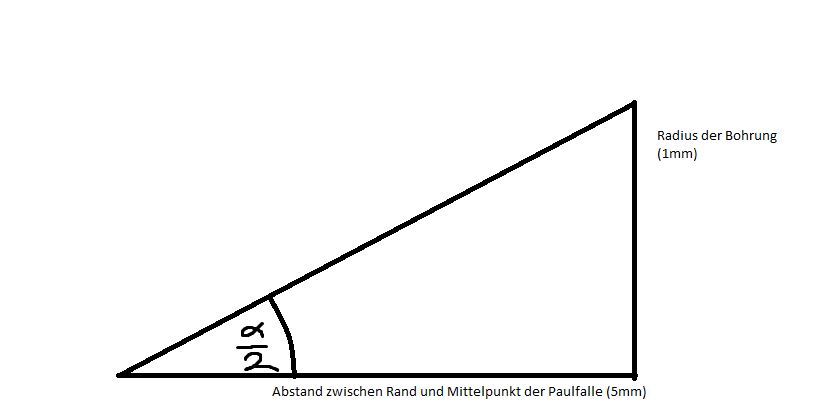
\includegraphics[scale = 0.5]{tan.png}
	\centering
	\caption{Geometrie des Strahlenganges innerhalb der Paulfalle}
	\label{optical_cavities}
\end{figure}
Somit gibt uns $tan(\alpha/2) = \frac{1mm}{5mm} \Rightarrow \alpha = 22,62°$ den Winkel $\alpha$, über welchen wir den Parameter Grad pro Pixel bestimmen konnten (0.03 $\frac{Grad}{Pixel}$). Anschließend haben wir einen zentralen Bildausschnitt gewählt um Randeffekte zu minimieren. Der über den Grad pro Pixel berechnete Ausschnitt lag zwischen den Winkeln 83,3° und 95,4°.  \\Im Aufnahmeprogramm hatten wir in periodischen Zeitabständen mehrere Bilder der Intensitätsverteilung aufgenommen und werteten die, am wenigsten Verrauschten, aus. \begin{figure}[h]
	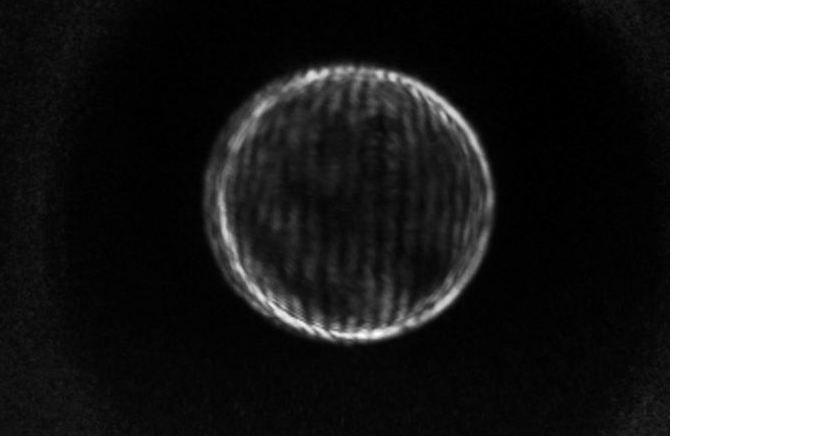
\includegraphics[scale = 0.5]{Abbild.png}
	\centering
	\caption{Bild der Intensitätsverteilung eines levitierten Teilchens}
	\label{optical_cavities}
\end{figure}
In Abbildung 6 sieht man das Bild der Intensitätsverteilung eines levitierten Teilchens. Im verwendeten Auswertungsprogramm konnten wir über die Parameter des Brechungsindexes und der Winkelverteilung die Radien des Tröpfchens mit Hilfe der Mie-Theorie berechnen. Dazu verglich das Programm die gemessene Verteilung mit denen möglicher Radien und gab die Übereinstimmung (Korrelation) aus. Den Radius haben wir für den Wert mit der höchsten Korrelation angenommen. Wir haben die Radien für zwei verschiedene Tröpfchen untersucht und folgende Werte in Table 3 (für Tröpfchen 1) und Table 4 (Tröpfchen 2) erhalten.

\begin{table}[h!]
	\centering
	\caption{Tröpfchen 1}
	\label{my-label}
	\begin{tabular}{ll}
		Zeit (t in s) & Radius (r in $\mu m$) \\
		0             & 11.45                \\
		17            & 9.74                 \\
		37            & 9.57                 \\
		57            & 8.16                 \\
		73            & 6.18                 \\
		92            & 7.54                 \\
		112           & 5.82                 \\
		128           & 5.51                
	\end{tabular}
\end{table}
\begin{table}[h!]
	\centering
	\caption{Tröpfchen 2}
	\label{my-label}
	\begin{tabular}{ll}
		Zeit (t in s) & Radius (r in $\mu m$) \\
		0             & 16.85                \\
		16            & 15.63                \\
		32            & 13.8                 \\
		75            & 12.22                \\
		87            & 11.93                \\
		108           & 10.83                \\
		126           & 11.11                \\
		148           & 9.41                 \\
		164           & 9.41                 \\
		183           & 8.02                 \\
		222           & 7.85                 \\
		239           & 7.85                
	\end{tabular}
\end{table}
\\Für die Radien haben wir einen Fehler $\Delta r = 1\mu m$ angenommen und über die Lineare Regression in Python den Verdampfungsparameter S bestimmt. Dafür haben wir zunächst die Radien quadriert um den Zusammenhang $r^{2} = r_{0}^{2} - S*t$ darstellen zu können. Aus dieser Formel lässt sich ableiten, das der Radius proportional zur Wurzel der Zeit ist.
\begin{figure}[h]
	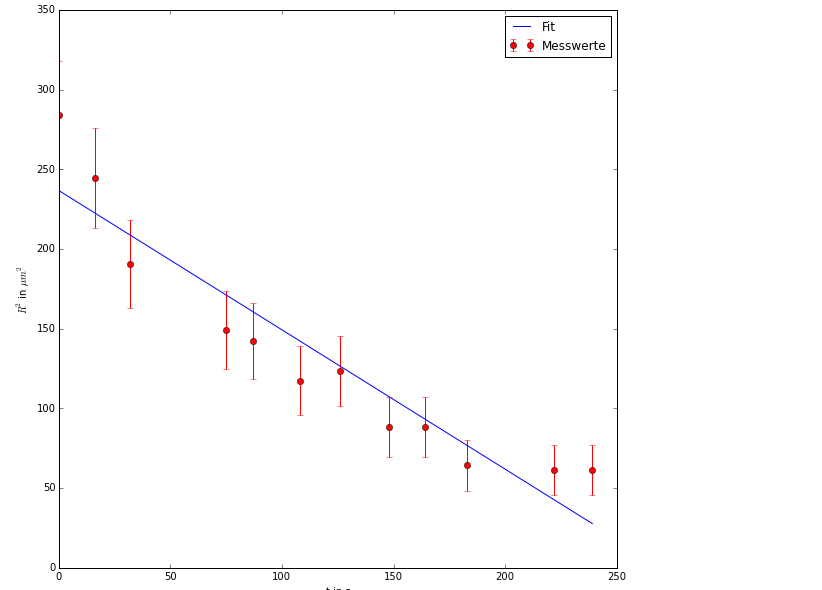
\includegraphics[scale = 0.5]{Graph1.png}
	\centering
	\caption{Abnahme des Radius für Tröpfchen 1}
	\label{optical_cavities}
\end{figure}
\begin{figure}[h]
	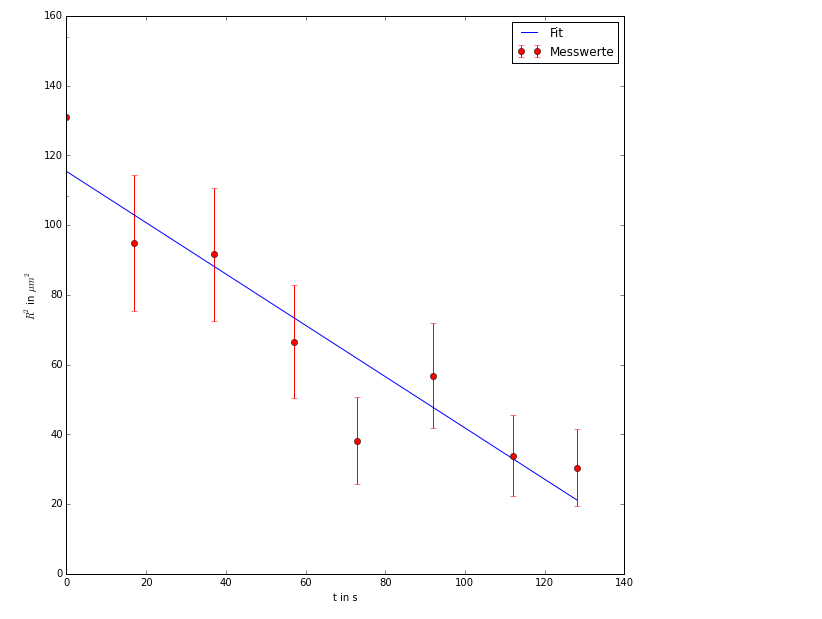
\includegraphics[scale = 0.5]{Graph2.png}
	\centering
	\caption{Abnahme des Radius für Tröpfchen 1}
	\label{optical_cavities}
\end{figure}
Aus unseren Fits haben wir die Verdampfungsparameter $S_{1}$ und $S_{2}$ mit dazugehöriger Standardabweichung und die Anfangsradien $r_{0}$ ermittelt:
$$ S_{1} = (8.74 \pm 0.98) *10^{-13} \frac{m^{2}}{s} $$ 
$$r_{01} = (15.38 \pm 0.50) \mu m$$
$$  S_{2} = (7.36 \pm 1.11) *10^{-13} \frac{m^{2}}{s}$$
$$ r_{02} = (10.74 \pm 0.50) \mu m $$
Die Lebensdauer des Tröpfchens lässt sich über den Schnittpunkt der Geraden mit der X-Achse berechnen. Durch Umstellen der Ausgangsgleichung erhält man:
$$ 0 = r_{0}^{2} - S*t \Rightarrow t_{R=0} =  \frac{r_{0}^{2}}{S} $$
Dies führt zu den Lebensdauern $t_{1}$ und $t_{2}$ für Tröpfchen 1/2:
$$ t_{1} = 270.64 \pm 35.52)s $$
$$ t_{2} = 156.72 \pm 27.77)s $$
Den Fehler für die Lebensdauern haben wir aus der Gaußschen Fehlerfortpflanzung berechnet. Des weiteren sollten wir eine Aussage darüber treffen, ob die Verdampfungsgeschwindigkeit von der momentanen Tröpfchengröße abhängt. Dafür gucken wir uns die zeitliche Änderung des Tröpfchenradius an, was wir als Verdampfungsgeschwindigkeit annehmen können:
$$\frac{\partial r(t)}{\partial t} = -\frac{S}{2} * \frac{1}{r(t)}$$
Somit ist die Verdampfungsgeschwindigkeit proportional zu 1/r vom momentanen Radius des Tröpfchens abhängig.

\section{Diskussion}

Es erwies sich als schwierig, geladene Glaskügelchen in der Paul-Falle gefangen zu halten. Nur bei zwei Kügelchen war uns dies über mehrere Messungen gelungen. An diesem Kügelchen bestimmten wir die spezifische Ladungen und, zusammenhängend mit dem Stabilitätsdiagramm der Paul-Falle, die Werte für a und q.
Nur eine der beiden Kugeln erwies sich als geeignet, um $\frac{Q}{m}$, a und q zu untersuchen. Ihr Wert für die spezifische Ladung betrug $(4,6 \pm 0,4)*10^{-3} \frac{kg}{C}$. Dieser Wert lässt sich nicht mit Literaturwerten vergleichen, weil er für jede Kugel zufällig ist. Nur in der Größenordnung der spezifischen Ladung könnten die Kugeln mit einem solchen Wert übereinstimmen.\\\\Wir untersuchten stabile Bereiche für die Glaskügelchen in der Paul-Falle und fanden mithilfe des Diagramms in Abbildung \ref{stabiler_bereich1} heraus, dass unsere gemessenen Werte für stabile Glaskügelchen dem theoretischen Stabilitätsdiagramm nicht widersprechen. Wegen der geringen Anzahl an Messpunkten konnten wir die Form des Stabilitätsdiagramms experimentell nicht überprüfen. Weil keine Messpunkte am Rand des theoretischen stabilen Bereichs gemessen werden konnten, ist es möglich, dass der tatsächliche stabile Bereich im Experiment kleiner, als in der Theorie, ist. Dies könnte auf Fehlerquellen im Experiment zurückzuführen sein. Mögliche Ursachen wären ein nicht stabiler Messaufbau oder Elektroden, dessen Form von der theoretischen Paul-Falle abweichen. Auch muss berücksichtigt werden, dass die Glaskügelchen nicht punktförmig sind. Dadurch könnte das Stabilitätsdiagramm anders aussehen.\\\\Für die Verdampfung levitierter Flüßigkeitstropfen ließ sich der vorher beschriebene Zusammenhang aufzeigen. Die ermittelten Werte für die Verdampfungsparameter $S_{1} = (8.74 \pm 0.98) *10^{-13} \frac{m^{2}}{s}$ und $S_{2} = (7.36 \pm 1.11) *10^{-13} \frac{m^{2}}{s}$ liegen jeweils im dreifachen Fehlerintervall des anderen Wertes. 
\end{document}